% Options for packages loaded elsewhere
\PassOptionsToPackage{unicode}{hyperref}
\PassOptionsToPackage{hyphens}{url}
\documentclass[
]{article}
\usepackage{xcolor}
\usepackage{amsmath,amssymb}
\setcounter{secnumdepth}{-\maxdimen} % remove section numbering
\usepackage{iftex}
\ifPDFTeX
  \usepackage[T1]{fontenc}
  \usepackage[utf8]{inputenc}
  \usepackage{textcomp} % provide euro and other symbols
\else % if luatex or xetex
  \usepackage{unicode-math} % this also loads fontspec
  \defaultfontfeatures{Scale=MatchLowercase}
  \defaultfontfeatures[\rmfamily]{Ligatures=TeX,Scale=1}
\fi
\usepackage{lmodern}
\ifPDFTeX\else
  % xetex/luatex font selection
\fi
% Use upquote if available, for straight quotes in verbatim environments
\IfFileExists{upquote.sty}{\usepackage{upquote}}{}
\IfFileExists{microtype.sty}{% use microtype if available
  \usepackage[]{microtype}
  \UseMicrotypeSet[protrusion]{basicmath} % disable protrusion for tt fonts
}{}
\makeatletter
\@ifundefined{KOMAClassName}{% if non-KOMA class
  \IfFileExists{parskip.sty}{%
    \usepackage{parskip}
  }{% else
    \setlength{\parindent}{0pt}
    \setlength{\parskip}{6pt plus 2pt minus 1pt}}
}{% if KOMA class
  \KOMAoptions{parskip=half}}
\makeatother
\usepackage{longtable,booktabs,array}
\usepackage{calc} % for calculating minipage widths
% Correct order of tables after \paragraph or \subparagraph
\usepackage{etoolbox}
\makeatletter
\patchcmd\longtable{\par}{\if@noskipsec\mbox{}\fi\par}{}{}
\makeatother
% Allow footnotes in longtable head/foot
\IfFileExists{footnotehyper.sty}{\usepackage{footnotehyper}}{\usepackage{footnote}}
\makesavenoteenv{longtable}
\usepackage{graphicx}
\makeatletter
\newsavebox\pandoc@box
\newcommand*\pandocbounded[1]{% scales image to fit in text height/width
  \sbox\pandoc@box{#1}%
  \Gscale@div\@tempa{\textheight}{\dimexpr\ht\pandoc@box+\dp\pandoc@box\relax}%
  \Gscale@div\@tempb{\linewidth}{\wd\pandoc@box}%
  \ifdim\@tempb\p@<\@tempa\p@\let\@tempa\@tempb\fi% select the smaller of both
  \ifdim\@tempa\p@<\p@\scalebox{\@tempa}{\usebox\pandoc@box}%
  \else\usebox{\pandoc@box}%
  \fi%
}
% Set default figure placement to htbp
\def\fps@figure{htbp}
\makeatother
\ifLuaTeX
  \usepackage{luacolor}
  \usepackage[soul]{lua-ul}
\else
  \usepackage{soul}
\fi
% definitions for citeproc citations
\NewDocumentCommand\citeproctext{}{}
\NewDocumentCommand\citeproc{mm}{%
  \begingroup\def\citeproctext{#2}\cite{#1}\endgroup}
\makeatletter
 % allow citations to break across lines
 \let\@cite@ofmt\@firstofone
 % avoid brackets around text for \cite:
 \def\@biblabel#1{}
 \def\@cite#1#2{{#1\if@tempswa , #2\fi}}
\makeatother
\newlength{\cslhangindent}
\setlength{\cslhangindent}{1.5em}
\newlength{\csllabelwidth}
\setlength{\csllabelwidth}{3em}
\newenvironment{CSLReferences}[2] % #1 hanging-indent, #2 entry-spacing
 {\begin{list}{}{%
  \setlength{\itemindent}{0pt}
  \setlength{\leftmargin}{0pt}
  \setlength{\parsep}{0pt}
  % turn on hanging indent if param 1 is 1
  \ifodd #1
   \setlength{\leftmargin}{\cslhangindent}
   \setlength{\itemindent}{-1\cslhangindent}
  \fi
  % set entry spacing
  \setlength{\itemsep}{#2\baselineskip}}}
 {\end{list}}
\usepackage{calc}
\newcommand{\CSLBlock}[1]{\hfill\break\parbox[t]{\linewidth}{\strut\ignorespaces#1\strut}}
\newcommand{\CSLLeftMargin}[1]{\parbox[t]{\csllabelwidth}{\strut#1\strut}}
\newcommand{\CSLRightInline}[1]{\parbox[t]{\linewidth - \csllabelwidth}{\strut#1\strut}}
\newcommand{\CSLIndent}[1]{\hspace{\cslhangindent}#1}
\setlength{\emergencystretch}{3em} % prevent overfull lines
\providecommand{\tightlist}{%
  \setlength{\itemsep}{0pt}\setlength{\parskip}{0pt}}
\usepackage{bookmark}
\IfFileExists{xurl.sty}{\usepackage{xurl}}{} % add URL line breaks if available
\urlstyle{same}
\hypersetup{
  pdftitle={AGENTE CONVERSACIONAL PARA INTERAÇÃO APRIMORADA EM SISTEMAS},
  hidelinks,
  pdfcreator={LaTeX via pandoc}}

\title{\textbf{AGENTE CONVERSACIONAL PARA INTERAÇÃO APRIMORADA EM
SISTEMAS}}
\author{}
\date{}

\begin{document}
\maketitle

\textbf{Lucas de Castro Zanoni}\footnote{Graduando em Engenharia de
  software no semestre letivo de 2024-2. E-mail:
  castro.lucas290@gmail.com}

\textbf{Thyerri Fernandes Mezzari}\footnote{Professor do Centro
  Universitário UniSATC E-mail: thyerri.mezzari@satc.edu.br}

Resumo: Este trabalho apresenta o desenvolvimento de um agente
conversacional baseado em inteligência artificial para aprimorar a
interação entre usuários e sistemas. Utilizando técnicas avançadas de
processamento de linguagem natural, o agente proposto visa simplificar a
comunicação em interfaces complexas, proporcionando uma experiência
digital unificada e adaptável às necessidades dos usuários. A
metodologia inclui o desenvolvimento, implementação e avaliação do
agente em ambientes reais de uso. Os resultados demonstram que a solução
proposta contribui significativamente para a melhoria da acessibilidade
e usabilidade dos sistemas, reduzindo barreiras de interação e
promovendo uma comunicação mais fluida e intuitiva.

\textbf{Palavras-chaves:} agente conversacional, interação, sistema,
inteligência artificial.

\textbf{1 INTRODUÇÃO}

\textbf{O trabalho de conclusão de curso deverá conter no mínimo 15 e no
máximo 30 páginas,} distribuídas nos tópicos Resumo; 1. Introdução; 2.
Procedimento Experimental, 2.1 Materiais, 2.2 Métodos; 3. Resultados e
Discussões, 4. Considerações Finais, Agradecimentos (se houver) e
Referências. A de quantidade máxima de páginas em cada tópico não tem
regra.

O texto introdutório precisa ser claro e objetivo. Você precisará expor,
de forma sucinta, a natureza da pesquisa, assim como a intenção desta.
De forma sutil, deverá apresentar as informações da pesquisa e, por
isso, a importância de a introdução ser elaborada ao final da escrita do
artigo.

Esta etapa do trabalho servirá para você apresentar ao leitor a sua
pesquisa, o tema, incentivando-o e motivando-o à leitura. É importante
lembrar de que a introdução não deve parafrasear ou repetir o resumo.

Procure responder nesta seção: - Por que estudar o tema escolhido?; -
Quais as vantagens e os benefícios que a pesquisa irá proporcionar?; -
Como ela contribuirá com a sociedade ou com uma parte dela?).

\textbf{O que se faz?} Caracteriza-se o problema de pesquisa
(pergunta-problema), bem como o

Nesta etapa (objetivo geral e os objetivos específicos) você deverá
responder a seguinte pergunta: Com que finalidade estou fazendo este
estudo? O objetivo geral deve descrever de modo claro e sucinto uma meta
a ser atingida e ser capaz de explicar o que você realmente deseja obter
com o estudo. Lembre-se que os objetivos precisarão iniciar com os
verbos no infinitivo. Exemplos de verbos: avaliar, analisar, aplicar,
comparar, considerar, demonstrar, desenvolver, reconhecer, usar,
assumir, julgar, prever, reforçar, entre outros.

Contém a ideia central do trabalho, e é apresentado em até três ou
quatro linhas.

Os objetivos específicos são para você detalhar as etapas que seguirá
para alcançar o objetivo geral. Para isso, você pensará no seguinte: de
que informações eu preciso para alcançar o objetivo geral? Assim como no
objetivo geral, os objetivos específicos precisarão iniciar com os
verbos no infinitivo.

Não devem apresentar as etapas de realização do trabalho, ou as etapas
do procedimento. Os objetivos específicos devem ser escritos com base
nas conclusões que se espera obter com o trabalho. Por exemplo: muitos
alunos escreve um objetivo específico como ``realizar a \ul{distribuição
granulométrica}'' enquanto deveria ser ``avaliar o \ul{efeito do tamanho
de partícula} sobre a resistência mecânica''.

Em seguida, devem ser expostas as justificativas e as razões para a
elaboração do trabalho, dando ênfase à relevância do tema proposto.

A justificativa, como o próprio nome indica, procura explicar por que o
trabalho é fundamental e relevante. O tema escolhido pelo pesquisador e
a hipótese levantada precisam ser de suma importância para a sociedade
ou para uma parte dela. Deve-se, no entanto, tomar o cuidado, na
elaboração da justificativa, de não se tentar justificar a hipótese
levantada, ou seja, ser uma conclusão da pesquisa.

A justificativa exalta a importância do tema a ser estudado e justifica
o porquê de a pesquisa ter sido empreendida. Ela difere de uma revisão
bibliográfica e, por esse motivo, não apresenta citações de outros
autores, apenas busca ressaltar a importância da pesquisa no campo da
teoria.

Procure responder nesta etapa: Por que estudar o tema escolhido? Quais
as vantagens e os benefícios que a pesquisa irá proporcionar? Qual a
importância pessoal? Qual a importância para a academia, a ciência? Qual
a importância para o mercado de trabalho? Como ela contribuirá com a
sociedade ou com uma parte dela?

\section*{2 PROCEDIMENTO EXPERIMENTAL}\label{procedimento-experimental}
\addcontentsline{toc}{section}{2 PROCEDIMENTO EXPERIMENTAL}

Nesta seção, deve-se descrever o procedimento experimental adotado. Seja
um procedimento experimental realizado em laboratório ou os critérios
analisados para o estudo do caso em questão, dentre outros. Lembrando
que este tópico será dividido em 2.1 MATERIAIS e 2.2 MÉTODOS, ou seja,
todos os recursos utilizados para a avaliação da pesquisa.

2.1 MATERIAIS (SUBTÍTULO SEÇÃO SECUNDÁRIA)

Esta seção deve indicar os recursos utilizados para realizar a pesquisa.
Deve, portanto, apresentar os materiais utilizados na pesquisa o tamanho
da amostra e como ela foi determinada.

2.2 MÉTODOS (SUBTÍTULO SEÇÃO SECUNDÁRIA)

Em métodos deve ter uma explicação minuciosa, detalhada, rigorosa e
exata de toda ação desenvolvida no método (caminho) do trabalho de
pesquisa. É necessário descrever quais equipamentos serão utilizados e
todo o procedimento experimental.

É a explicação do tipo de pesquisa, do instrumental utilizado
(softwares, equipamentos, questionários, entrevistas, etc.), do tempo
previsto, do laboratório, das formas de tabulação e tratamento dos
dados, enfim, de tudo aquilo que se utilizou ou será utilizado no
trabalho.

\textbf{A seguir regras de formatação para o desenvolvimento do artigo:}

É de extrema importância realizar uma pesquisa bibliográfica, do tema a
ser estudado, baseada em periódicos nacionais e internacionais (artigos,
anais de congressos, revistas especializadas) e também em livros, teses
e dissertações para direcionar os procedimentos experimetais adotados e
os resultados e discussões obtidos. Essas referências deveram ser
citadas ao longo do artigo.

É importante compreender que cópias de trechos deverão ser feitas de
acordo com as normas da ABNT, ou seja: citações diretas e/ou indiretas,
curtas e/ou longas. Cópia de trechos e/ou na íntegra sem os devidos
créditos é considerado plágio (lei nº 9.610, de 19.02.98, que altera,
atualiza e consolida a legislação sobre direitos autorais). Não se
esqueça de nomear a seção.

O trabalho deve ter formato A4 (21 cm × 29,7 cm), digitado em espaço de
1,5. A fonte utilizada deverá ser Arial, em corpo 12 para o texto, em
corpo 10 para as citações longas e igualmente 10 para as notas de
rodapé.

Margens: para superior e esquerda 3 cm, inferior e direita 2,0 cm.

Recuo de primeira linha dos parágrafos: 2 cm.

O número da página deve vir na parte superior da página, à direita.

\textbf{O trabalho deve ser escrito totalmente na 3ª pessoa do singular
e/ou plural.}

O título do trabalho deve ser apresentado em letra maiúscula,
centralizado e negritado.

O nome do autor deve ser alinhado à direita da página, em letra
minúscula e negrito. Para a identificação deve-se usar nota de rodapé
que deve conter a titulação e o e-mail.

Os capítulos devem ser divididos de acordo com as necessidades do autor.
A seção primária deve ser apresentada em caixa alta e negrito; a seção
secundária deve ser em caixa alta e sem negrito. A seção terciária deve
ser apresentada em letra minúscula e com negrito.

Os títulos devem ser separados do texto com um espaço de 1,5 e não devem
ficar separados do texto caso ocorra uma quebra de página.

As siglas deverão vir acompanhadas do nome por extenso na primeira vez
que são citadas no texto.

O uso de negrito deve ficar restrito aos títulos, e o itálico, apenas
para destacar conceitos ou grifar palavras estrangeiras.

Quando o pesquisador produz a imagem, a tabela, o quadro é necessário
especificar a fonte. Exemplo: Do autor (2025).

Figuras, quadros e tabelas devem ser inseridos no corpo do texto com
legendas em tamanho 12 e centralizados e com espaçamento simples.

As imagens devem ser de boa qualidade e legíveis.

Nas figuras, quadros e tabelas o título deverá vir acima, ser numerado
de forma crescente e apresentar a fonte de pesquisa (tamanho 10) abaixo.

As unidades de medidas deverão seguir o Sistema Internacional de
Unidades.

\textbf{3.1.1 Seção terciária} (usar título relacionado ao tema)

Entre a figura, a tabela, o quadro e a equação e o texto que o antecede
e o sucede, deve-se usar um espaço de 1,5.

A figura deve ser inserida centralizada e próxima do trecho a que se
refere, conforme o projeto gráfico. Preferencialmente, insira figuras e
tabelas após elas serem citadas no texto. Use a abreviação figura 1 para
chamar no texto, mesmo no início de uma frase. Veja, a seguir, o exemplo
com figuras:

\begin{quote}
Figura 1: Biblioteca virtual Pearson.
\end{quote}

\begin{figure}
\centering
\pandocbounded{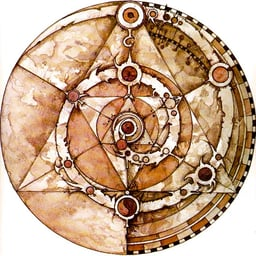
\includegraphics[keepaspectratio]{./images/image-test.jpg}}
\caption{Biblioteca virtual Pearson}
\end{figure}

\begin{quote}
Fonte: Baseado e/ou Adaptado de (Silva 2018)

Figura 2: Nuvem de palavras.
\end{quote}

\begin{figure}
\centering
\pandocbounded{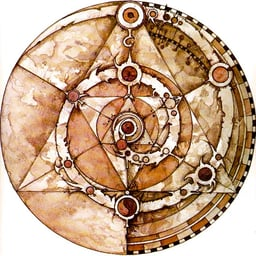
\includegraphics[keepaspectratio]{./images/image-test.jpg}}
\caption{Nuvem de palavras}
\end{figure}

\begin{quote}
Fonte: (Pacheco 2018)
\end{quote}

Gráficos são considerados figuras. Veja, a seguir, o gráfico para
exemplificar:

\begin{quote}
Figura 2: Sistema de cascata.
\end{quote}

\begin{figure}
\centering
\pandocbounded{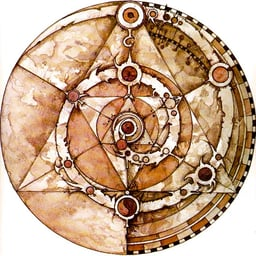
\includegraphics[keepaspectratio]{./images/image-test.jpg}}
\caption{Sistema de cascata}
\end{figure}

Fonte: Adaptado de (Fonseca 2005, 61)

Use palavras ao invés de símbolos ou abreviações para evitar confundir o
leitor. Como um exemplo, escrever a quantidade ``Magnetização'' ou
``Magnetização, M'', e não apenas ``M''. Se incluir unidades no rótulo,
apresentá-las dentro de parênteses. Não rotule os eixos somente com
unidades. No exemplo, escreva ``Magnetização (A/m)'' e não apenas
``A/m''.

Dentro da tabela e do quadro utilize fonte em tamanho 10. Veja, agora,
exemplos com tabela, tabela. 1 e tabela. 2:

\begin{quote}
Tabela 1: Melhor configuração (tensão constante).
\end{quote}

Variáveis

Valores Otimizados

(sem saturação)

Fator de Potência

0,7000

Torque Médio (N.m)

15,3934

Ângulo de Carga (graus)

33,6239

Espessura da barreira (mm)

1,9999

Ld (mH)

289,8727

Lq(mH)

56,3546

Ld/Lq

5,1437

Ld-Lq (mH)

233,5180

Fonte: Baseado e/ou Adaptado de (Silva 2018, 10)

Tabela 2: Produção de uvas no Brasil, em toneladas.

\begin{longtable}[]{@{}llll@{}}
\toprule\noalign{}
\textbf{Estado/ano} & \textbf{2013} & \textbf{2014} & \textbf{2015} \\
\midrule\noalign{}
\endhead
\bottomrule\noalign{}
\endlastfoot
Ceará & 664 & 573 & 940 \\
Pernambuco & 228.727 & 236.767 & 237.376 \\
\end{longtable}

Fonte: Do autor (2018)

Exemplo de quadro, quadro 1:

Quadro 1: Gêneros e aparatos de edição do jornal.

Gêneros

Aparatos de Edição

Presos:

Editorial

Carta do leitor

Expediente

Chamada

Índice

Cabeçalho

Livres:

Notícia

Nota

Crítica

Comentário

Opinião

Reportagem

Entrevista

Claquete

Manchete

Lide

Lista

Painel

Chapéu

Olho

Tabela

Gráfico

Citação

Exemplo

Perfil

Selo

Fonte: (Bonini 2001)

Exemplo do uso de equação, utiliza-se a equação (1):

\begin{longtable}[]{@{}ll@{}}
\toprule\noalign{}
\(AT = \frac{n \times N \times 1000}{V}\) & (1) \\
\midrule\noalign{}
\endhead
\bottomrule\noalign{}
\endlastfoot
\end{longtable}

Onde:

AT = acidez total (meq/L);

n = volume da solução de hidróxido de sódio gastos na titulação (mL);

N = normalidade da solução de hidróxido de sódio (N);

V = volume da amostra (mL).

Quando em uma equação for citada uma grandeza adimensional, é necessário
especificar desta forma:

Onde:

Re = número de Reynolds (-\/-\/-);

As reações químicas ao longo do texto devem ser mencionadas conforme
exemplo a seguir. Não sendo necessário deixar um espaço entre a reação
química e o texto.

A reação de formação da água é representada pela Reação (1).

\begin{longtable}[]{@{}ll@{}}
\toprule\noalign{}
\(H_{2} + \frac{1}{2}O_{2} \rightarrow H_{2}O\) & (1) \\
\midrule\noalign{}
\endhead
\bottomrule\noalign{}
\endlastfoot
\end{longtable}

Ao mencionar tabelas, figuras, quadros e equações no texto, os mesmos
devem vir abreviados: Fig., Tab., Qd., Eq.

Veja, a seguir, um texto com alíneas:

O questionário será organizado a partir de três critérios, a saber:

\begin{enumerate}
\def\labelenumi{\alph{enumi})}
\item
  idade:

  \begin{itemize}
  \item
    de 30 a 40 anos;
  \item
    mais de 40 anos.
  \end{itemize}
\item
  sexo;
\item
  estado civil.
\end{enumerate}

As citações devem seguir o padrão da ABNT NBR 10520/2023.

\begin{itemize}
\tightlist
\item
  Citação indireta (paráfrase).
\end{itemize}

A citação indireta trata-se de uma reprodução das ideias de um autor com
outras palavras. Para fazer uma citação indireta leia e releia o texto
original até que seja capaz de reescrevê-lo com suas próprias palavras;
não use aspas nas citações indiretas/paráfrases; anote os dados
referentes à fonte: sobrenome do autor, seguido do ano de publicação da
obra.

Atenção: quando a obra apresentar mais de três autores, indica-se apenas
o primeiro, acrescentando-se a expressão et al.

Exemplos:

A fim de garantir que seu passado seja preservado e salvaguardado, a
criação de um acervo fotográfico permitirá a disseminação da história e
da memória institucional (Sousa, Fujita, and Gracioso 2014).

Segundo Sousa, Fujita, and Gracioso (2014), a fim de garantir que seu
passado seja preservado e salvaguardado, a criação de um acervo
fotográfico permitirá a disseminação da história e da memória
institucional.

\begin{itemize}
\tightlist
\item
  Citação direta curta (até 03 linhas) -- cópia literal:
\end{itemize}

O acervo fotográfico, ``visa contribuir para o processo do que deve se
tornar memorável em âmbito institucional'' (Mendonça and Pinho 2016,
91).

\begin{itemize}
\tightlist
\item
  Citação direta longa (mais de 03 linhas) - cópia literal:
\end{itemize}

Segundo Filippi, Lima, and Carvalho (2002, 11):

\begin{quote}
Nos últimos vinte anos, a fotografia deixou definitivamente de ser um
mero instrumento ilustrativo da pesquisa para assumir o status de
documento, uma matéria-prima fundamental na produção do conhecimento
sobre determinados períodos da história, acontecimentos e grupos
sociais.
\end{quote}

Em caso de dúvidas, consulte a ABNT NBR 10520/2023 que se refere a
``Informações e documentação -- citações em documentos''.

O autor deverá escolher a forma de apresentação das referências:

\begin{itemize}
\item
  \textbf{ordem alfabética}: as referências devem ser reunidas no final
  do artigo em uma única ordem alfabética por sobrenome do autor;
\item
  \textbf{ordem numérica}: as referências devem seguir a mesma ordem
  numérica crescente utilizada no texto.
\end{itemize}

\begin{itemize}
\item
  As referências devem vir reunidas no final do artigo em uma única
  ordem (alfabética ou numérica)
\item
  Todos os endereços de páginas na internet (URLs) incluídas no texto
  deverão estar ativos e prontos para o acesso;
\item
  Referência alinhada à esquerda, espaçamento simples, separadas por
  dois (2) espaços simples;
\item
  Quando tratar de consulta on-line, será necessário indicar o endereço
  eletrônico e a data em que foi acessado, se a obra estiver em suporte
  eletrônico (DVD, CD-ROM), esta informação também deve constar após a
  sua identificação;
\item
  Para referência de documentos consultar a ABNT 6023;
\item
  As citações e referências utilizadas nesse manual são meramente
  ilustrativas.
\end{itemize}

\textbf{3 RESULTADOS E DISCUSSÕES}

Nos Resultados e Discussões, deve-se apresentar os resultados obtidos no
Procedimento Experimental e fazer uma discussão e análise sobre os
mesmos sempre que possível referenciando a literatura pesquisada.

\textbf{4 CONSIDERAÇÕES FINAIS}

Etapa esta que servirá para você evidenciar as conquistas alcançadas com
o estudo e indicar as limitações e as reconsiderações. Além disso, você
poderá apontar a relação entre fatos verificados e teoria e mostrar a
contribuição da pesquisa para o meio acadêmico, empresarial e/ou para o
desenvolvimento da ciência e tecnologia. Além disso, você poderá sugerir
temas complementares a sua pesquisa para estudos futuros. Responda aqui
a sua pergunta-problema de pesquisa.

\section{REFERÊNCIAS \{\#referências
.9-Títulos-pós-textuais\}}\label{referuxeancias-referuxeancias-.9-tuxedtulos-puxf3s-textuais}

\hl{Exemplo numérico:}

{[}1{]} MARCONI, Marina de Andrade; LAKATOS, Eva Maria.
\textbf{Fundamentos de metodologia científica. }7. ed.~São Paulo: Atlas,
2010. 297 p.~ISBN 9788522457588.

{[}2{]} ALBUQUERQUE, Ana Cristina de. \textbf{Catalogação e descrição de
documentos fotográficos em bibliotecas e arquivos}: uma aproximação
comparativa dos códigos AACR2 e ISAD (G). 2006. 188f. Dissertação
(Mestrado) -- Faculdade de Filosofia e Ciências, Universidade Estadual
Paulista, Marília, 2006. Disponível em: \textless{}
https://www.marilia.unesp.br/Home/Pos-Graduacao/CienciadaInformacao/Dissertacoes/albuquerque\_ac\_me\_mar.pdf\textgreater.
Acesso em: 12 setembro 2017.

{[}3{]} RAUEN, Fábio José. \textbf{Roteiros de pesquisa}. Rio do Sul:
Nova Era, 2006.

{[}4{]} BONINI, A.; et al\emph{.} Mídia, suporte e hipergênero: os
gêneros textuais e suas relações. \textbf{Revista Brasileira de
Linguística Aplicada}. Belo Horizonte, v. 11, n.~3, p.~679-704, 2011.

{[}5{]} MARCONI, Marina de Andrade. Cultura e sociedade. In: LAKATOS,
Eva Maria. \textbf{Sociologia}\emph{.} 6. ed.~São Paulo: Atlas, 1991.

{[}6{]} ALCÂNTARA, Eurípedes. A redoma do atraso. \textbf{Veja}\emph{,}
São Paulo, v. 24, n.~25, p.~42-43, jun. 1991.

{[}7{]} RIBEIRO, Efrém. Garimpeiros voltam a invadir área ianomani.
\textbf{Folha de S. Paulo}\emph{,} São Paulo, p.~1-10, 18 jun. 1991.

\hl{Exemplo alfabético:}

ALCÂNTARA, Eurípedes. A redoma do atraso. \textbf{Veja}\emph{,} São
Paulo, v. 24, n.~25, p.~42-43, jun. 1991.

BONINI, A.; et al\emph{.} Mídia, suporte e hipergênero: os gêneros
textuais e suas relações. \textbf{Revista Brasileira de Linguística
Aplicada}. Belo Horizonte, v. 11, n.~3, p.~679-704, 2011.

MARCONI, Marina de Andrade. Cultura e sociedade. In: LAKATOS, Eva Maria.
\textbf{Sociologia}\emph{.} 6. ed.~São Paulo: Atlas, 1991.

MARCONI, Marina de Andrade; LAKATOS, Eva Maria. \textbf{Fundamentos de
metodologia científica. }7. ed.~São Paulo: Atlas, 2010. 297 p.~ISBN
9788522457588.

RIBEIRO, Efrém. Garimpeiros voltam a invadir área ianomani.
\textbf{Folha de S. Paulo}\emph{,} São Paulo, p.~1-10, 18 jun. 1991.

RAUEN, Fábio José. \textbf{Roteiros de pesquisa}. Rio do Sul: Nova Era,
2006.

\textbf{AGRADECIMENTOS}

Este item é opcional e deve conter no máximo 5 linhas. Além de poder
agradecer a pessoas que contribuíram para a realização do trabalho, é
possível agradecer empresas e financiadores.

\textbf{LISTA DE SÍMBOLOS}

A lista de símbolos deve ser utilizada somente quanto o trabalho conter
muitas equações. Caso necessário é possível que a lista de símbolos
contenha duas colunas e o tamanho da letra seja 10.

\begin{longtable}[]{@{}
  >{\raggedright\arraybackslash}p{(\linewidth - 6\tabcolsep) * \real{0.3056}}
  >{\raggedright\arraybackslash}p{(\linewidth - 6\tabcolsep) * \real{0.1667}}
  >{\raggedright\arraybackslash}p{(\linewidth - 6\tabcolsep) * \real{0.4583}}
  >{\raggedright\arraybackslash}p{(\linewidth - 6\tabcolsep) * \real{0.0694}}@{}}
\toprule\noalign{}
\begin{minipage}[b]{\linewidth}\raggedright
\[\beta\]
\end{minipage} & \begin{minipage}[b]{\linewidth}\raggedright
{[}K\textsuperscript{-1}{]}
\end{minipage} & \begin{minipage}[b]{\linewidth}\raggedright
Coeficiente de expansão térmica
\end{minipage} & \begin{minipage}[b]{\linewidth}\raggedright
\end{minipage} \\
\midrule\noalign{}
\endhead
\bottomrule\noalign{}
\endlastfoot
\(\mathrm{\Delta}T\) & {[}K{]} & Variação de temperatura & \\
\(\eta_{a}\) & {[}-\/-\/-{]} & Eficiência da aleta & \\
\(\nu\) & {[}m\textsuperscript{2}/s{]} & Viscosidade cinemática & \\
\(A_{c}\) & {[}m\textsuperscript{2}{]} & Área da seção transversal & \\
\(A_{sp}\) & {[}m\textsuperscript{2}{]} & Área da superfície da placa
& \\
\(\cos\theta\) & {[}-\/-\/-{]} & Fator de potência & \\
\(d\) & {[}m{]} & Braço de momento & \\
\(F\) & {[}N{]} & Força de momento & \\
\(g\) & {[}m/s\textsuperscript{2}{]} & Aceleração da gravidade & \\
\end{longtable}

\phantomsection\label{refs}
\begin{CSLReferences}{1}{0}
\bibitem[\citeproctext]{ref-Bonini2001}
Bonini, Adair. 2001. {``Mídia, Suporte e Hipergênero: Os Gêneros
Textuais e Suas Relações.''} \emph{Revista Brasileira de Linguística
Aplicada} 11 (3): 679--704.

\bibitem[\citeproctext]{ref-Filippi2002}
Filippi, Patrícia, Solange Ferraz Lima, and Vânia Carneiro Carvalho.
2002. \emph{Como Tratar Coleções de Fotografias}. São Paulo: Arquivo do
Estado.

\bibitem[\citeproctext]{ref-Fonseca2005}
Fonseca, João José Saraiva da. 2005. \emph{Metodologia Da Pesquisa
Científica}. Fortaleza: UECE.

\bibitem[\citeproctext]{ref-Mendonca2016}
Mendonça, Ricardo Rodrigues, and Fábio Assis Pinho. 2016. {``Fotografia
e Memória Organizacional: Um Estudo de Caso Em Uma Instituição
Pública.''} \emph{Perspectivas Em Ciência Da Informação} 21 (3):
88--102.

\bibitem[\citeproctext]{ref-Pacheco2018}
Pacheco, Maria Teresa. 2018. {``Análise de Dados Qualitativos Em
Pesquisas Científicas.''} \emph{Revista Brasileira de Pesquisa
Qualitativa} 6 (2): 113--29.

\bibitem[\citeproctext]{ref-Silva2018}
Silva, João Carlos da. 2018. \emph{Metodologia Da Pesquisa Aplicada}.
São Paulo: Editora Atlas.

\bibitem[\citeproctext]{ref-Sousa2014}
Sousa, Ana Paula, Mariângela Spotti Lopes Fujita, and Luciana de Souza
Gracioso. 2014. {``Acervos Fotográficos e Memória Institucional: Métodos
e Técnicas de Preservação.''} \emph{Revista Brasileira de
Biblioteconomia e Documentação} 10 (1): 58--73.

\end{CSLReferences}

\end{document}
